\documentclass[]{article}
\usepackage{lmodern}
\usepackage{amssymb,amsmath}
\usepackage{ifxetex,ifluatex}
\usepackage{fixltx2e} % provides \textsubscript
\ifnum 0\ifxetex 1\fi\ifluatex 1\fi=0 % if pdftex
  \usepackage[T1]{fontenc}
  \usepackage[utf8]{inputenc}
\else % if luatex or xelatex
  \ifxetex
    \usepackage{mathspec}
  \else
    \usepackage{fontspec}
  \fi
  \defaultfontfeatures{Ligatures=TeX,Scale=MatchLowercase}
\fi
% use upquote if available, for straight quotes in verbatim environments
\IfFileExists{upquote.sty}{\usepackage{upquote}}{}
% use microtype if available
\IfFileExists{microtype.sty}{%
\usepackage{microtype}
\UseMicrotypeSet[protrusion]{basicmath} % disable protrusion for tt fonts
}{}
\usepackage[margin=1in]{geometry}
\usepackage{hyperref}
\hypersetup{unicode=true,
            pdftitle={DATA 606 - Lab 3},
            pdfauthor={Joshua Sturm},
            pdfborder={0 0 0},
            breaklinks=true}
\urlstyle{same}  % don't use monospace font for urls
\usepackage{color}
\usepackage{fancyvrb}
\newcommand{\VerbBar}{|}
\newcommand{\VERB}{\Verb[commandchars=\\\{\}]}
\DefineVerbatimEnvironment{Highlighting}{Verbatim}{commandchars=\\\{\}}
% Add ',fontsize=\small' for more characters per line
\usepackage{framed}
\definecolor{shadecolor}{RGB}{248,248,248}
\newenvironment{Shaded}{\begin{snugshade}}{\end{snugshade}}
\newcommand{\KeywordTok}[1]{\textcolor[rgb]{0.13,0.29,0.53}{\textbf{{#1}}}}
\newcommand{\DataTypeTok}[1]{\textcolor[rgb]{0.13,0.29,0.53}{{#1}}}
\newcommand{\DecValTok}[1]{\textcolor[rgb]{0.00,0.00,0.81}{{#1}}}
\newcommand{\BaseNTok}[1]{\textcolor[rgb]{0.00,0.00,0.81}{{#1}}}
\newcommand{\FloatTok}[1]{\textcolor[rgb]{0.00,0.00,0.81}{{#1}}}
\newcommand{\ConstantTok}[1]{\textcolor[rgb]{0.00,0.00,0.00}{{#1}}}
\newcommand{\CharTok}[1]{\textcolor[rgb]{0.31,0.60,0.02}{{#1}}}
\newcommand{\SpecialCharTok}[1]{\textcolor[rgb]{0.00,0.00,0.00}{{#1}}}
\newcommand{\StringTok}[1]{\textcolor[rgb]{0.31,0.60,0.02}{{#1}}}
\newcommand{\VerbatimStringTok}[1]{\textcolor[rgb]{0.31,0.60,0.02}{{#1}}}
\newcommand{\SpecialStringTok}[1]{\textcolor[rgb]{0.31,0.60,0.02}{{#1}}}
\newcommand{\ImportTok}[1]{{#1}}
\newcommand{\CommentTok}[1]{\textcolor[rgb]{0.56,0.35,0.01}{\textit{{#1}}}}
\newcommand{\DocumentationTok}[1]{\textcolor[rgb]{0.56,0.35,0.01}{\textbf{\textit{{#1}}}}}
\newcommand{\AnnotationTok}[1]{\textcolor[rgb]{0.56,0.35,0.01}{\textbf{\textit{{#1}}}}}
\newcommand{\CommentVarTok}[1]{\textcolor[rgb]{0.56,0.35,0.01}{\textbf{\textit{{#1}}}}}
\newcommand{\OtherTok}[1]{\textcolor[rgb]{0.56,0.35,0.01}{{#1}}}
\newcommand{\FunctionTok}[1]{\textcolor[rgb]{0.00,0.00,0.00}{{#1}}}
\newcommand{\VariableTok}[1]{\textcolor[rgb]{0.00,0.00,0.00}{{#1}}}
\newcommand{\ControlFlowTok}[1]{\textcolor[rgb]{0.13,0.29,0.53}{\textbf{{#1}}}}
\newcommand{\OperatorTok}[1]{\textcolor[rgb]{0.81,0.36,0.00}{\textbf{{#1}}}}
\newcommand{\BuiltInTok}[1]{{#1}}
\newcommand{\ExtensionTok}[1]{{#1}}
\newcommand{\PreprocessorTok}[1]{\textcolor[rgb]{0.56,0.35,0.01}{\textit{{#1}}}}
\newcommand{\AttributeTok}[1]{\textcolor[rgb]{0.77,0.63,0.00}{{#1}}}
\newcommand{\RegionMarkerTok}[1]{{#1}}
\newcommand{\InformationTok}[1]{\textcolor[rgb]{0.56,0.35,0.01}{\textbf{\textit{{#1}}}}}
\newcommand{\WarningTok}[1]{\textcolor[rgb]{0.56,0.35,0.01}{\textbf{\textit{{#1}}}}}
\newcommand{\AlertTok}[1]{\textcolor[rgb]{0.94,0.16,0.16}{{#1}}}
\newcommand{\ErrorTok}[1]{\textcolor[rgb]{0.64,0.00,0.00}{\textbf{{#1}}}}
\newcommand{\NormalTok}[1]{{#1}}
\usepackage{graphicx,grffile}
\makeatletter
\def\maxwidth{\ifdim\Gin@nat@width>\linewidth\linewidth\else\Gin@nat@width\fi}
\def\maxheight{\ifdim\Gin@nat@height>\textheight\textheight\else\Gin@nat@height\fi}
\makeatother
% Scale images if necessary, so that they will not overflow the page
% margins by default, and it is still possible to overwrite the defaults
% using explicit options in \includegraphics[width, height, ...]{}
\setkeys{Gin}{width=\maxwidth,height=\maxheight,keepaspectratio}
\IfFileExists{parskip.sty}{%
\usepackage{parskip}
}{% else
\setlength{\parindent}{0pt}
\setlength{\parskip}{6pt plus 2pt minus 1pt}
}
\setlength{\emergencystretch}{3em}  % prevent overfull lines
\providecommand{\tightlist}{%
  \setlength{\itemsep}{0pt}\setlength{\parskip}{0pt}}
\setcounter{secnumdepth}{0}
% Redefines (sub)paragraphs to behave more like sections
\ifx\paragraph\undefined\else
\let\oldparagraph\paragraph
\renewcommand{\paragraph}[1]{\oldparagraph{#1}\mbox{}}
\fi
\ifx\subparagraph\undefined\else
\let\oldsubparagraph\subparagraph
\renewcommand{\subparagraph}[1]{\oldsubparagraph{#1}\mbox{}}
\fi

%%% Use protect on footnotes to avoid problems with footnotes in titles
\let\rmarkdownfootnote\footnote%
\def\footnote{\protect\rmarkdownfootnote}

%%% Change title format to be more compact
\usepackage{titling}

% Create subtitle command for use in maketitle
\newcommand{\subtitle}[1]{
  \posttitle{
    \begin{center}\large#1\end{center}
    }
}

\setlength{\droptitle}{-2em}
  \title{DATA 606 - Lab 3}
  \pretitle{\vspace{\droptitle}\centering\huge}
  \posttitle{\par}
  \author{Joshua Sturm}
  \preauthor{\centering\large\emph}
  \postauthor{\par}
  \predate{\centering\large\emph}
  \postdate{\par}
  \date{09/13/2017}


\begin{document}
\maketitle

In this lab we'll investigate the probability distribution that is most
central to statistics: the normal distribution. If we are confident that
our data are nearly normal, that opens the door to many powerful
statistical methods. Here we'll use the graphical tools of R to assess
the normality of our data and also learn how to generate random numbers
from a normal distribution.

\subsection{The Data}\label{the-data}

This week we'll be working with measurements of body dimensions. This
data set contains measurements from 247 men and 260 women, most of whom
were considered healthy young adults.

\begin{Shaded}
\begin{Highlighting}[]
\KeywordTok{load}\NormalTok{(}\KeywordTok{url}\NormalTok{(}\StringTok{"http://www.openintro.org/stat/data/bdims.RData"}\NormalTok{))}
\KeywordTok{data}\NormalTok{(bdims.RData)}
\end{Highlighting}
\end{Shaded}

\begin{verbatim}
## Warning in data(bdims.RData): data set 'bdims.RData' not found
\end{verbatim}

Let's take a quick peek at the first few rows of the data.

\begin{Shaded}
\begin{Highlighting}[]
\KeywordTok{head}\NormalTok{(bdims)}
\end{Highlighting}
\end{Shaded}

\begin{verbatim}
##   bia.di bii.di bit.di che.de che.di elb.di wri.di kne.di ank.di sho.gi
## 1   42.9   26.0   31.5   17.7   28.0   13.1   10.4   18.8   14.1  106.2
## 2   43.7   28.5   33.5   16.9   30.8   14.0   11.8   20.6   15.1  110.5
## 3   40.1   28.2   33.3   20.9   31.7   13.9   10.9   19.7   14.1  115.1
## 4   44.3   29.9   34.0   18.4   28.2   13.9   11.2   20.9   15.0  104.5
## 5   42.5   29.9   34.0   21.5   29.4   15.2   11.6   20.7   14.9  107.5
## 6   43.3   27.0   31.5   19.6   31.3   14.0   11.5   18.8   13.9  119.8
##   che.gi wai.gi nav.gi hip.gi thi.gi bic.gi for.gi kne.gi cal.gi ank.gi
## 1   89.5   71.5   74.5   93.5   51.5   32.5   26.0   34.5   36.5   23.5
## 2   97.0   79.0   86.5   94.8   51.5   34.4   28.0   36.5   37.5   24.5
## 3   97.5   83.2   82.9   95.0   57.3   33.4   28.8   37.0   37.3   21.9
## 4   97.0   77.8   78.8   94.0   53.0   31.0   26.2   37.0   34.8   23.0
## 5   97.5   80.0   82.5   98.5   55.4   32.0   28.4   37.7   38.6   24.4
## 6   99.9   82.5   80.1   95.3   57.5   33.0   28.0   36.6   36.1   23.5
##   wri.gi age  wgt   hgt sex
## 1   16.5  21 65.6 174.0   1
## 2   17.0  23 71.8 175.3   1
## 3   16.9  28 80.7 193.5   1
## 4   16.6  23 72.6 186.5   1
## 5   18.0  22 78.8 187.2   1
## 6   16.9  21 74.8 181.5   1
\end{verbatim}

You'll see that for every observation we have 25 measurements, many of
which are either diameters or girths. A key to the variable names can be
found at \url{http://www.openintro.org/stat/data/bdims.php}, but we'll
be focusing on just three columns to get started: weight in kg
(\texttt{wgt}), height in cm (\texttt{hgt}), and \texttt{sex}
(\texttt{1} indicates male, \texttt{0} indicates female).

Since males and females tend to have different body dimensions, it will
be useful to create two additional data sets: one with only men and
another with only women.

\begin{Shaded}
\begin{Highlighting}[]
\NormalTok{mdims <-}\StringTok{ }\KeywordTok{subset}\NormalTok{(bdims, sex ==}\StringTok{ }\DecValTok{1}\NormalTok{)}
\NormalTok{fdims <-}\StringTok{ }\KeywordTok{subset}\NormalTok{(bdims, sex ==}\StringTok{ }\DecValTok{0}\NormalTok{)}
\end{Highlighting}
\end{Shaded}

\begin{enumerate}
\def\labelenumi{\arabic{enumi}.}
\tightlist
\item
  Make a histogram of men's heights and a histogram of women's heights.
  How would you compare the various aspects of the two distributions?
\end{enumerate}

\subsection{The normal distribution}\label{the-normal-distribution}

In your description of the distributions, did you use words like
\emph{bell-shaped} or \emph{normal}? It's tempting to say so when faced
with a unimodal symmetric distribution.

To see how accurate that description is, we can plot a normal
distribution curve on top of a histogram to see how closely the data
follow a normal distribution. This normal curve should have the same
mean and standard deviation as the data. We'll be working with women's
heights, so let's store them as a separate object and then calculate
some statistics that will be referenced later.

\begin{Shaded}
\begin{Highlighting}[]
\NormalTok{fhgtmean <-}\StringTok{ }\KeywordTok{mean}\NormalTok{(fdims$hgt)}
\NormalTok{fhgtsd   <-}\StringTok{ }\KeywordTok{sd}\NormalTok{(fdims$hgt)}
\end{Highlighting}
\end{Shaded}

Next we make a density histogram to use as the backdrop and use the
\texttt{lines} function to overlay a normal probability curve. The
difference between a frequency histogram and a density histogram is that
while in a frequency histogram the \emph{heights} of the bars add up to
the total number of observations, in a density histogram the
\emph{areas} of the bars add up to 1. The area of each bar can be
calculated as simply the height \emph{times} the width of the bar. Using
a density histogram allows us to properly overlay a normal distribution
curve over the histogram since the curve is a normal probability density
function. Frequency and density histograms both display the same exact
shape; they only differ in their y-axis. You can verify this by
comparing the frequency histogram you constructed earlier and the
density histogram created by the commands below.

\begin{Shaded}
\begin{Highlighting}[]
\KeywordTok{hist}\NormalTok{(fdims$hgt, }\DataTypeTok{probability =} \OtherTok{TRUE}\NormalTok{)}
\NormalTok{x <-}\StringTok{ }\DecValTok{140}\NormalTok{:}\DecValTok{190}
\NormalTok{y <-}\StringTok{ }\KeywordTok{dnorm}\NormalTok{(}\DataTypeTok{x =} \NormalTok{x, }\DataTypeTok{mean =} \NormalTok{fhgtmean, }\DataTypeTok{sd =} \NormalTok{fhgtsd)}
\KeywordTok{lines}\NormalTok{(}\DataTypeTok{x =} \NormalTok{x, }\DataTypeTok{y =} \NormalTok{y, }\DataTypeTok{col =} \StringTok{"blue"}\NormalTok{)}
\end{Highlighting}
\end{Shaded}

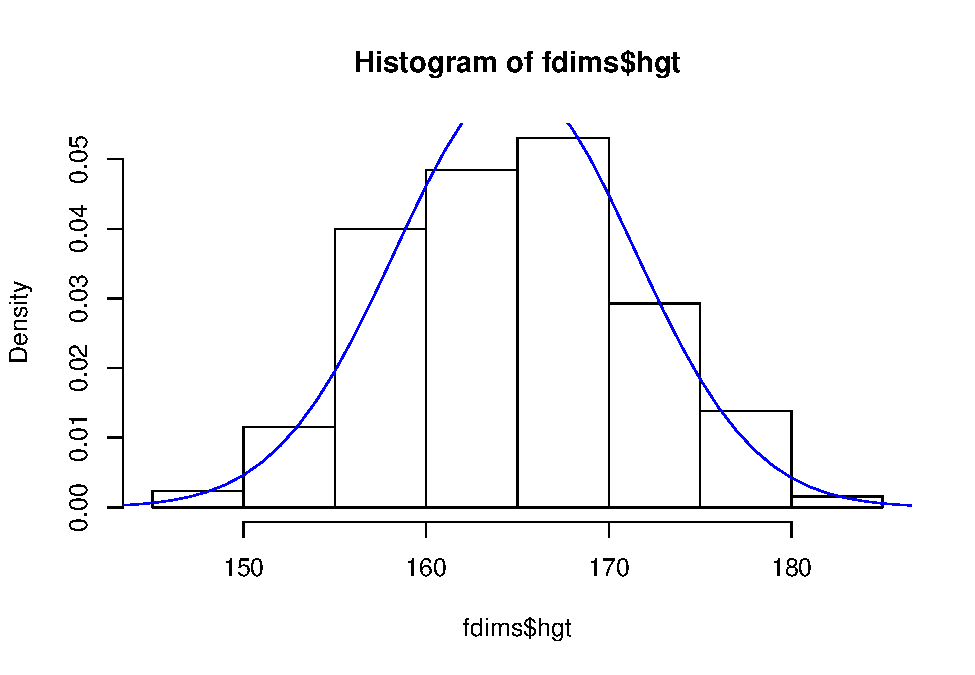
\includegraphics{DATA_606_-_Lab_3_files/figure-latex/hist-height-1.pdf}

After plotting the density histogram with the first command, we create
the x- and y-coordinates for the normal curve. We chose the \texttt{x}
range as 140 to 190 in order to span the entire range of
\texttt{fheight}. To create \texttt{y}, we use \texttt{dnorm} to
calculate the density of each of those x-values in a distribution that
is normal with mean \texttt{fhgtmean} and standard deviation
\texttt{fhgtsd}. The final command draws a curve on the existing plot
(the density histogram) by connecting each of the points specified by
\texttt{x} and \texttt{y}. The argument \texttt{col} simply sets the
color for the line to be drawn. If we left it out, the line would be
drawn in black.

The top of the curve is cut off because the limits of the x- and y-axes
are set to best fit the histogram. To adjust the y-axis you can add a
third argument to the histogram function: \texttt{ylim\ =\ c(0,\ 0.06)}.

\begin{enumerate}
\def\labelenumi{\arabic{enumi}.}
\setcounter{enumi}{1}
\tightlist
\item
  Based on the this plot, does it appear that the data follow a nearly
  normal distribution?
\end{enumerate}

\subsection{Evaluating the normal
distribution}\label{evaluating-the-normal-distribution}

Eyeballing the shape of the histogram is one way to determine if the
data appear to be nearly normally distributed, but it can be frustrating
to decide just how close the histogram is to the curve. An alternative
approach involves constructing a normal probability plot, also called a
normal Q-Q plot for ``quantile-quantile''.

\begin{Shaded}
\begin{Highlighting}[]
\KeywordTok{qqnorm}\NormalTok{(fdims$hgt)}
\KeywordTok{qqline}\NormalTok{(fdims$hgt)}
\end{Highlighting}
\end{Shaded}

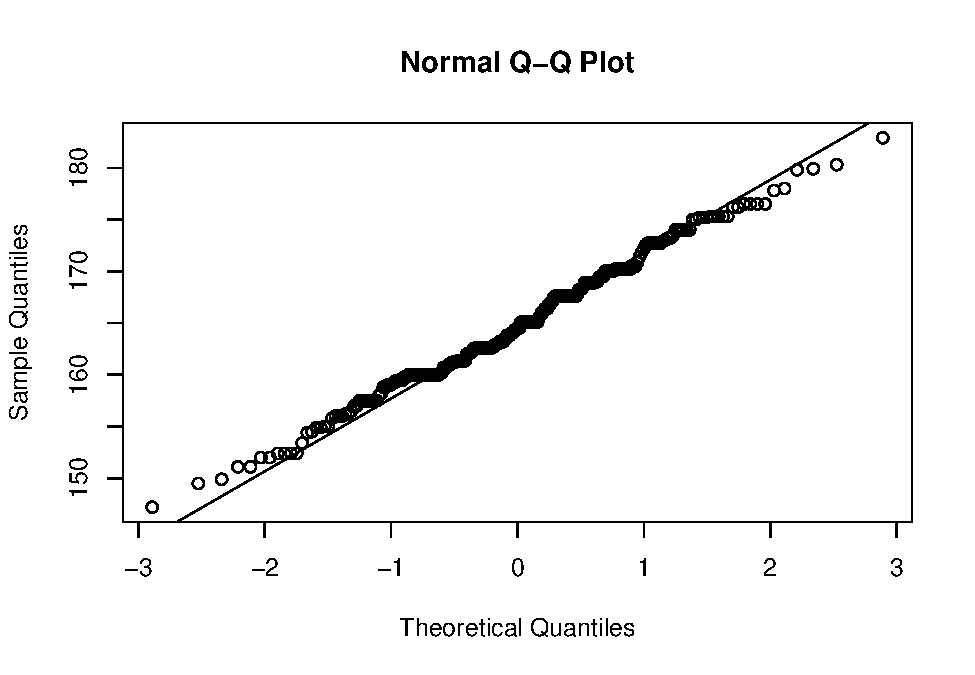
\includegraphics{DATA_606_-_Lab_3_files/figure-latex/qq-1.pdf}

A data set that is nearly normal will result in a probability plot where
the points closely follow the line. Any deviations from normality leads
to deviations of these points from the line. The plot for female heights
shows points that tend to follow the line but with some errant points
towards the tails. We're left with the same problem that we encountered
with the histogram above: how close is close enough?

A useful way to address this question is to rephrase it as: what do
probability plots look like for data that I \emph{know} came from a
normal distribution? We can answer this by simulating data from a normal
distribution using \texttt{rnorm}.

\begin{Shaded}
\begin{Highlighting}[]
\NormalTok{sim_norm <-}\StringTok{ }\KeywordTok{rnorm}\NormalTok{(}\DataTypeTok{n =} \KeywordTok{length}\NormalTok{(fdims$hgt), }\DataTypeTok{mean =} \NormalTok{fhgtmean, }\DataTypeTok{sd =} \NormalTok{fhgtsd)}
\end{Highlighting}
\end{Shaded}

The first argument indicates how many numbers you'd like to generate,
which we specify to be the same number of heights in the \texttt{fdims}
data set using the \texttt{length} function. The last two arguments
determine the mean and standard deviation of the normal distribution
from which the simulated sample will be generated. We can take a look at
the shape of our simulated data set, \texttt{sim\_norm}, as well as its
normal probability plot.

\begin{enumerate}
\def\labelenumi{\arabic{enumi}.}
\setcounter{enumi}{2}
\tightlist
\item
  Make a normal probability plot of \texttt{sim\_norm}. Do all of the
  points fall on the line? How does this plot compare to the probability
  plot for the real data?
\end{enumerate}

Even better than comparing the original plot to a single plot generated
from a normal distribution is to compare it to many more plots using the
following function. It may be helpful to click the zoom button in the
plot window.

\begin{Shaded}
\begin{Highlighting}[]
\KeywordTok{qqnormsim}\NormalTok{(fdims$hgt)}
\end{Highlighting}
\end{Shaded}

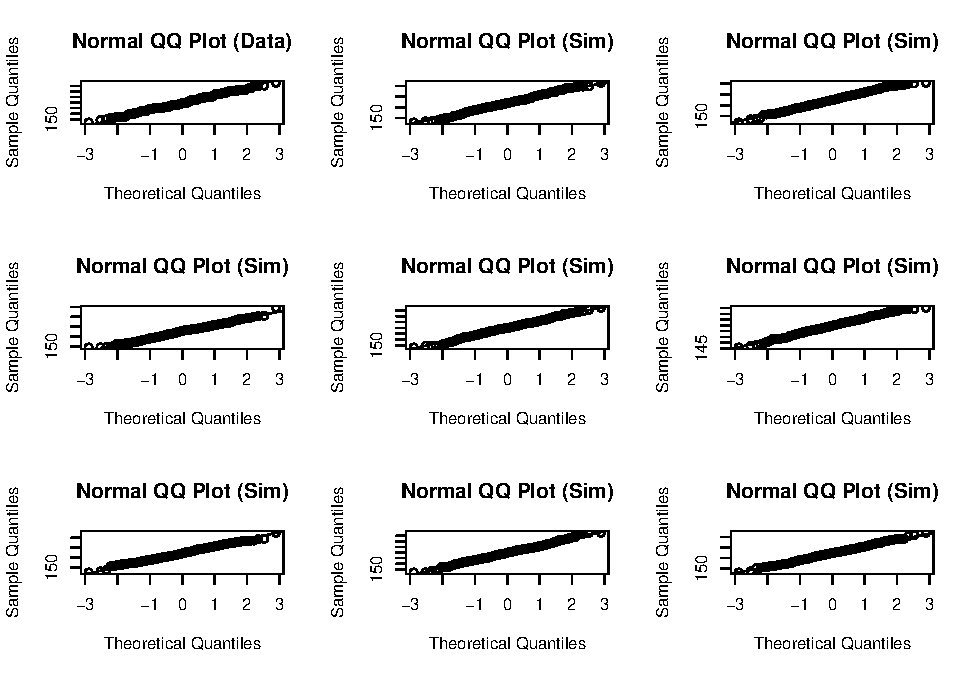
\includegraphics{DATA_606_-_Lab_3_files/figure-latex/qqnormsim-1.pdf}

\begin{enumerate}
\def\labelenumi{\arabic{enumi}.}
\setcounter{enumi}{3}
\item
  Does the normal probability plot for \texttt{fdims\$hgt} look similar
  to the plots created for the simulated data? That is, do plots provide
  evidence that the female heights are nearly normal?
\item
  Using the same technique, determine whether or not female weights
  appear to come from a normal distribution.
\end{enumerate}

\subsection{Normal probabilities}\label{normal-probabilities}

Okay, so now you have a slew of tools to judge whether or not a variable
is normally distributed. Why should we care?

It turns out that statisticians know a lot about the normal
distribution. Once we decide that a random variable is approximately
normal, we can answer all sorts of questions about that variable related
to probability. Take, for example, the question of, ``What is the
probability that a randomly chosen young adult female is taller than 6
feet (about 182 cm)?'' (The study that published this data set is clear
to point out that the sample was not random and therefore inference to a
general population is not suggested. We do so here only as an exercise.)

If we assume that female heights are normally distributed (a very close
approximation is also okay), we can find this probability by calculating
a Z score and consulting a Z table (also called a normal probability
table). In R, this is done in one step with the function \texttt{pnorm}.

\begin{Shaded}
\begin{Highlighting}[]
\DecValTok{1} \NormalTok{-}\StringTok{ }\KeywordTok{pnorm}\NormalTok{(}\DataTypeTok{q =} \DecValTok{182}\NormalTok{, }\DataTypeTok{mean =} \NormalTok{fhgtmean, }\DataTypeTok{sd =} \NormalTok{fhgtsd)}
\end{Highlighting}
\end{Shaded}

\begin{verbatim}
## [1] 0.004434387
\end{verbatim}

Note that the function \texttt{pnorm} gives the area under the normal
curve below a given value, \texttt{q}, with a given mean and standard
deviation. Since we're interested in the probability that someone is
taller than 182 cm, we have to take one minus that probability.

Assuming a normal distribution has allowed us to calculate a theoretical
probability. If we want to calculate the probability empirically, we
simply need to determine how many observations fall above 182 then
divide this number by the total sample size.

\begin{Shaded}
\begin{Highlighting}[]
\KeywordTok{sum}\NormalTok{(fdims$hgt >}\StringTok{ }\DecValTok{182}\NormalTok{) /}\StringTok{ }\KeywordTok{length}\NormalTok{(fdims$hgt)}
\end{Highlighting}
\end{Shaded}

\begin{verbatim}
## [1] 0.003846154
\end{verbatim}

Although the probabilities are not exactly the same, they are reasonably
close. The closer that your distribution is to being normal, the more
accurate the theoretical probabilities will be.

\begin{enumerate}
\def\labelenumi{\arabic{enumi}.}
\setcounter{enumi}{5}
\tightlist
\item
  Write out two probability questions that you would like to answer; one
  regarding female heights and one regarding female weights. Calculate
  the those probabilities using both the theoretical normal distribution
  as well as the empirical distribution (four probabilities in all).
  Which variable, height or weight, had a closer agreement between the
  two methods?
\end{enumerate}

\begin{center}\rule{0.5\linewidth}{\linethickness}\end{center}

\subsection{On Your Own}\label{on-your-own}

\begin{itemize}
\item
  Now let's consider some of the other variables in the body dimensions
  data set. Using the figures at the end of the exercises, match the
  histogram to its normal probability plot. All of the variables have
  been standardized (first subtract the mean, then divide by the
  standard deviation), so the units won't be of any help. If you are
  uncertain based on these figures, generate the plots in R to check.

  \textbf{a.} The histogram for female biiliac (pelvic) diameter
  (\texttt{bii.di}) belongs to normal probability plot letter \_\_\_\_.

  \textbf{b.} The histogram for female elbow diameter (\texttt{elb.di})
  belongs to normal probability plot letter \_\_\_\_.

  \textbf{c.} The histogram for general age (\texttt{age}) belongs to
  normal probability plot letter \_\_\_\_.

  \textbf{d.} The histogram for female chest depth (\texttt{che.de})
  belongs to normal probability plot letter \_\_\_\_.
\item
  Note that normal probability plots C and D have a slight stepwise
  pattern.\\
  Why do you think this is the case?
\item
  As you can see, normal probability plots can be used both to assess
  normality and visualize skewness. Make a normal probability plot for
  female knee diameter (\texttt{kne.di}). Based on this normal
  probability plot, is this variable left skewed, symmetric, or right
  skewed? Use a histogram to confirm your findings.
\end{itemize}

\begin{figure}[htbp]
\centering
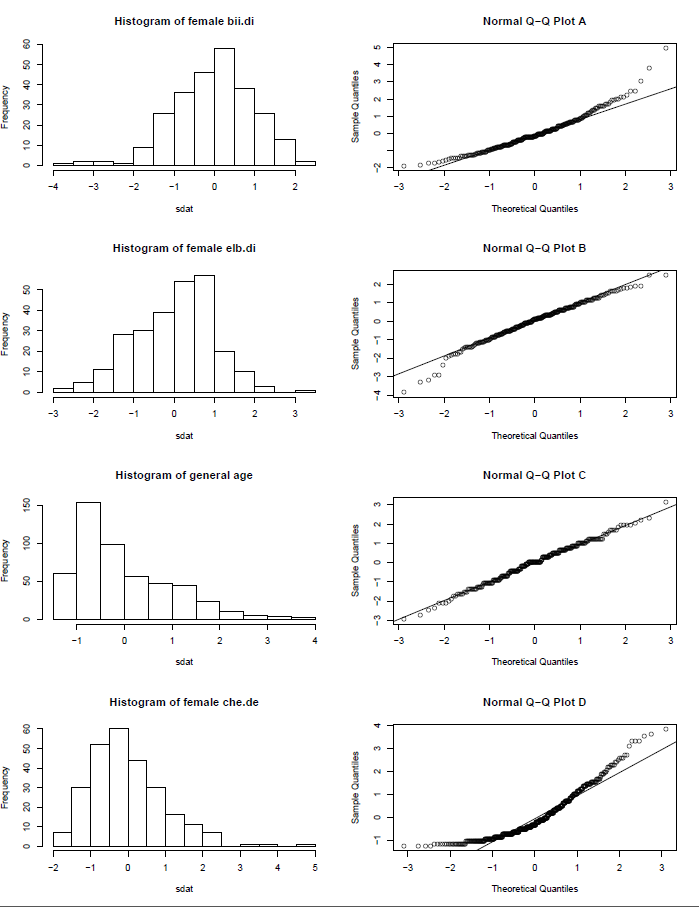
\includegraphics{more/histQQmatch.png}
\caption{histQQmatch}
\end{figure}

\hypertarget{license}{}
This is a product of OpenIntro that is released under a
\href{http://creativecommons.org/licenses/by-sa/3.0}{Creative Commons
Attribution-ShareAlike 3.0 Unported}. This lab was adapted for OpenIntro
by Andrew Bray and Mine Çetinkaya-Rundel from a lab written by Mark
Hansen of UCLA Statistics.


\end{document}
